\chapter{Discussion}
\label{sec:Discussion}
While the approach to applying IS-2's LiDAR measurements to ICEYE's SAR imaging was intuitive, there are several limitations of the experiment that should be acknowledged. These can be split into technical and conceptual limitations, where the former is responsible for immediate flaws in experimentation, and the latter can be viewed as persistent by nature of how they are related to the task. The practical implications of a working model are discussed after the limitations, and the section is concluded by future works for this project.

\section{Technical Limitations}
Limitations of the experimentation range from the data collection to the architecture and testing configuration. Firstly, the model's failure to converge was likely the result of inadequate architecture, but the restricted amount of data itself was plausibly a second limiting factor. As discussed at the end of the Data Collection section, of the 4 sponsored images delivered from ICEYE, only (Figure 2.2b) appeared to be correlated closely enough with IS-2's track to be considered ground truth. Despite efforts to validate the location and concentration of sea ice in the acquisition area by using Copernicus Access Hub, the selected area was too sparse for IS-2 to deliver information from all 6 beams. The low resolution of SN-2 data via Copernicus Access Hub combined with the latency between the data order and delivery means that there is a degree of randomness with any data acquisition even when sponsored. IS-2's data delivery flagged 70$\%$ of its gathered data for the possible interference of weather, either through blowing snow or clouds. Considering IS-2's weather flag then, the original expectation of $\approx$ 11,300 tiles from the 2 SPOT and 2 SLEA images actually only produced 1,391 tiles, for a yield of 12.30$\%$.

Furthermore with the data, the coincidence of (Figure 2.2b) is based on the assumption that the ice did not drift more than 17 meters within the acquisition window. Essentially, if the ice drifted even 3 $\frac{m}{min}$ it's possible for the data to be a close proxy for the ground truth, but technically incorrect altogether. Buoy data for the time frame showed that 2 buoys, 185km and 300km away were traveling at a mean speed of 12 $\frac{m}{min}$ and 16.67 $\frac{m}{min}$ respectively during the hour of acquisition. Combined with the assumed geolocation accuracy of 5m \cite{ICESat-2-Horizontal-Accuracy} and that some studies find the mean effective footprint of IS-2 to be 10.9 $\pm$ 1.2m\cite{icesatfootprintdiameter}, the assumption of coincidence becomes weaker.

Statistically, many measurements used during the study were accompanied by uncertanties, standard deviations, and confidence levels. These values were ignored during the experimentation, but should be considered in more thorough analysis in the future. 

\section{Conceptual Limitations}
The introduction discussed the assumption of hydrostatic equilibrium and associated Equation 1.1 as an established method to deduce ice thickness from remote measurements. Like previously mentioned, there is contention between which values to use for each density. Simply by assuming the maximum and minimum of acceptable densities for sea ice and snow, the same data from the experimentation can be seen ranging over a whole meter in some places like index 1050 (Figure 4.1). It's important to realize that this exact acquisition saw freeboard $<$ 1m, but with acquisitions of ice with more freeboard, these error bounds would increase in magnitude.

\begin{figure}[h]
	\centering
	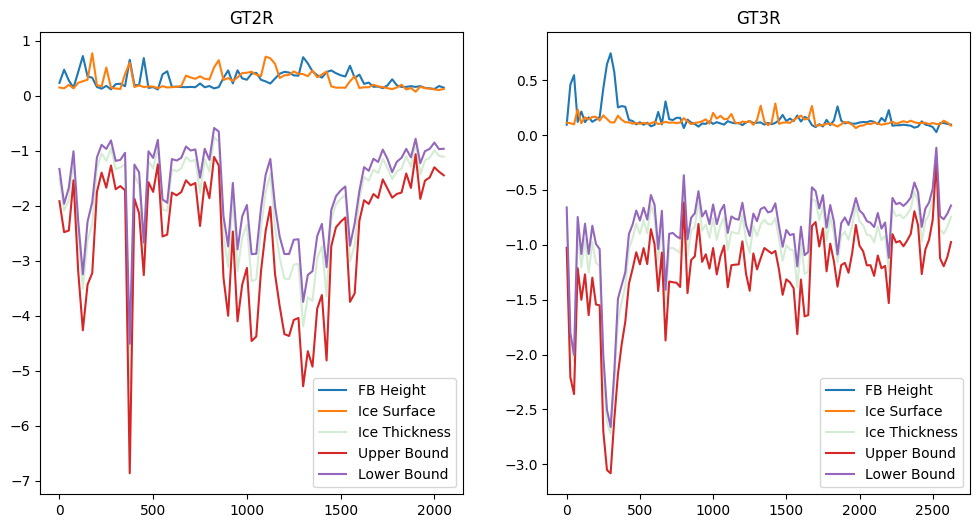
\includegraphics[width=.8\textwidth]{../research-resources/ice-sat-2/density-bounds.png}
	\caption[Effect of Density Estimations on Ice Thickness Interpolation]{Bounded Ice Thickness}
	\label{fig:density-bounds}
\end{figure}

Coupled with the issue of ice density in the hydrostatic model, is the general assumption of ice homogeneity. Figure 1.1 demonstrates the densities involved in interpolating for sea thickness, but it's important to realize these forces are assumed to be at play on independent buoyant ice segments. In practicality, ice floes as a whole are in hydrostatic equilibrium and the point-to-point assumption used in Figure 1.1 does not necessarily hold \cite{Forsström_Gerland_Pedersen_2011}. The differences can be results of ice deformation or composition, ridges, or even  internal shear forces \cite{Hutchings_Heil_Lecomte_Stevens_Steer_Lieser_2015,sea-ice-properties}. 

A final conceptual limitation with the corroboration of LiDAR with SAR imaging, is that the specific satellite capturing the image has a meaningful effect on the model being used. ICEYE's SAR imaging was pursued because of it's high 1m resolution. However, these images were captured using X-Band frequencies which are different from SN-2's \cite{iceye-products,Sentinel-2-Availability} frequencies. One of SAR's advantages is its ability to permeate through snow, allowing for it to capture the ice-surface below it. It's exact penetration depth though, is highly variable across the range RADAR \cite{remotesensingkinematics}. In this sense, the tiles derived from ICEYE will have to be compared to other X-Band SAR imaging satellites to ensure both images represent the same context.


\section{Practical Implications}
- Demo, does not need to be coded

\section{Future Work}
As mentioned in the experimentation, little work has been done in regression tasked CNNs of low resolution single channel images. The difficulty in aggregating a dataset for this study suggests that this task may not be a good use case for these deep learning models, as they rely heavily on mass amounts of data. However, the U-Net architecture is one such CNN that has seen efficacy in sea ice SAR imaging, particularly in image segmentation, and could be explored in its regression capabilites on lower-resolution images \cite{SAR-U-Net}. Moving forward, pursuing ensemble learning through a more statistical approach of the low resolution data would be a valuable use of the obtained data set, and possibly more feasible than a deep learning model.
